\documentclass[fleqn]{goose-article}

\title{Energy barrier}
\author{Tom de Geus}
\hypersetup{pdfauthor={T.W.J. de Geus}}

\begin{document}

\maketitle

\section*{Protocol}

The protocol is as follows.
\begin{enumerate}
    \item An element is selected for triggering
    (in the example below chosen in the center of the system).
    Its location is denoted by $\vec{r}'$.

    \item A perturbation around a stress and strain free configuration is considered.
    To this end, the selected element (only) is subjected to an eigen stress
    $\bm{\sigma}'$.
    The corresponding equilibrium configuration then constitutes to
    the perturbation that will be used.
    It is characterised by the stress field $\vec{u}^* (\vec{r})$, and corresponding
    stress $\bm{\sigma}^* (\vec{r})$
    and strain $\bm{\varepsilon}^* (\vec{r})$ fields.

    \item Two types of perturbations are considered:
    \begin{itemize}
        \item Simple shear:
        $\bm{\sigma}' = \bm{\sigma}'_s = \vec{e}_x \vec{e}_y + \vec{e}_x \vec{e}_y$.
        Gives: $\vec{u}^*_s (\vec{r})$, $\bm{\sigma}^*_s (\vec{r})$, and
        $\bm{\varepsilon}^*_s (\vec{r})$.

        \item Pure shear:
        $\bm{\sigma}' = \bm{\sigma}'_p = \vec{e}_x \vec{e}_x - \vec{e}_y \vec{e}_y$.
        Gives: $\vec{u}^*_p (\vec{r})$, $\bm{\sigma}^*_p (\vec{r})$, and
        $\bm{\varepsilon}^*_p (\vec{r})$.
    \end{itemize}

    For the triggered element the strain (and) stress are (by definition)
    of the following structure:
    $\bm{\varepsilon}^*_s (\vec{r}') = \chi_s (\vec{e}_x \vec{e}_y + \vec{e}_x \vec{e}_y)$
    for the simple shear perturbation, and
    $\bm{\varepsilon}^*_p (\vec{r}') = \chi_p (\vec{e}_x \vec{e}_x - \vec{e}_y \vec{e}_y)$
    for the pure shear perturbation.

    \item The two perturbative modes are scaled such that the energy increase to a perturbation
    with $\delta \vec{u}(\vec{r}) = s \vec{u}_s (\vec{r}) + p \vec{u}_p (\vec{r})$ is isotropic in
    the $(s, p)$-space.
    In particular, prefactors $\psi_s$ and $\psi_p$ are used to obtain
    \begin{equation}
        \vec{u}_i = \psi_i \vec{u}^*_i, \qquad
        \bm{\sigma}_i = \psi_i \bm{\sigma}^*_i, \qquad
        \bm{\varepsilon}_i = \psi_i \bm{\varepsilon}^*_i, \qquad
        \text{for}\; i \in (s, p)
    \end{equation}
    whereby
    \begin{itemize}
        \item Simple shear:
        $1 / \psi_s = (\sigma_{xy})^*_s (\varepsilon_{xy})^*_s$


        \item Simple shear:
        $1 / \psi_p = (\sigma_{yy})^*_p (\varepsilon_{yy})^*_p$
    \end{itemize}
    taking the stress and strain for the triggered element.

    The resulting perturbative displacement modes
    are shown in \cref{fig:perturbation},
    whereby the corresponding equivalent deviatoric stress is shown in colour.

    \item A perturbation with
    $\delta \vec{u}(\vec{r}) = s \vec{u}_s (\vec{r}) + p \vec{u}_p (\vec{r})$
    now results in an energy increase in the system that is isotropic in the $(s, p)$ domain,
    see \cref{fig:energy}.
    In contrast the increases in equivalent stress and strain span an ellipse
    in the $(s, p)$ domain, see \cref{fig:phase-diagram}.

\end{enumerate}

\begin{figure}[htp]
    \centering
    \captionsetup[subfigure]{justification=centering}
    \begin{minipage}[t]{.49\textwidth}
        \centering
        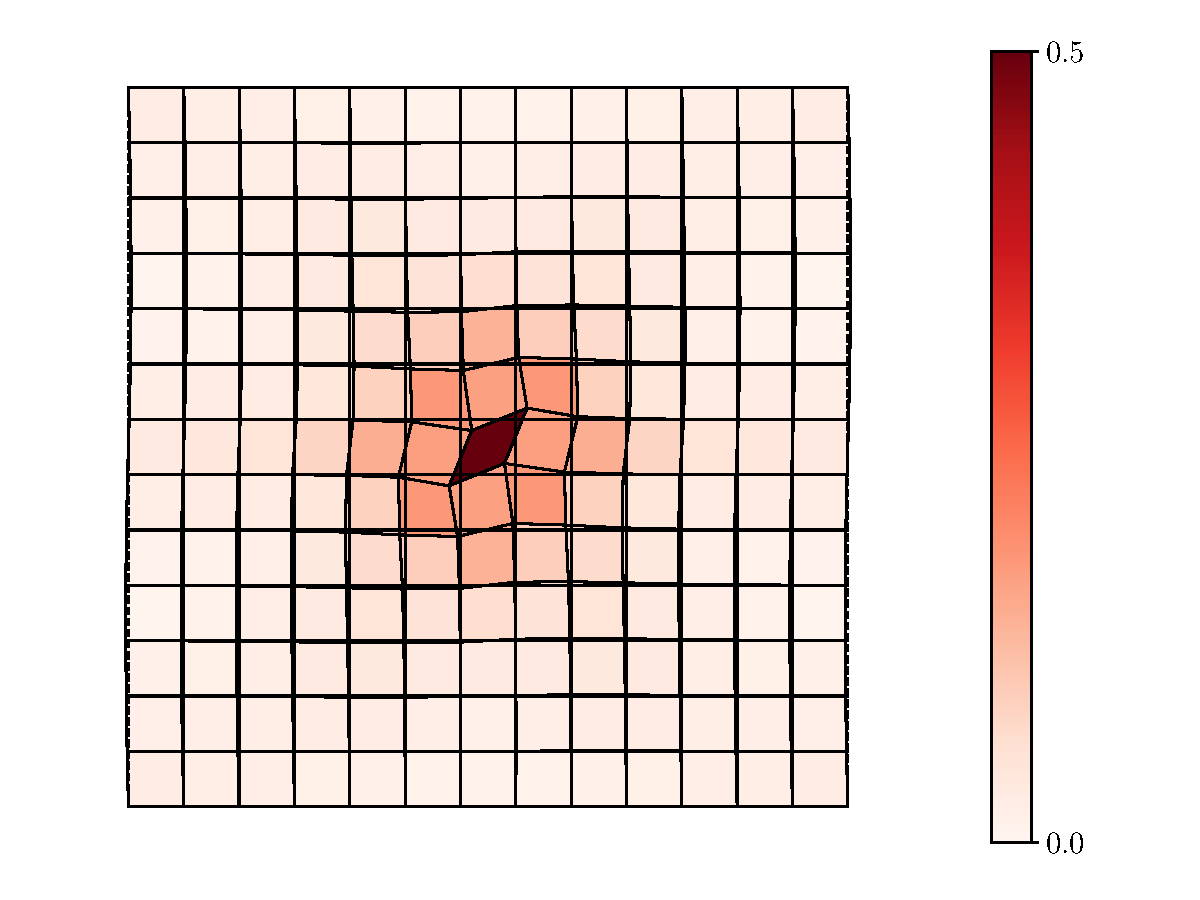
\includegraphics[width=\textwidth]{perturbation_simple-shear.pdf}
        \subcaption{Simple shear}
        \label{fig:perturbation:simple-shear}
    \end{minipage}
    \hfill
    \begin{minipage}[t]{.49\textwidth}
        \centering
        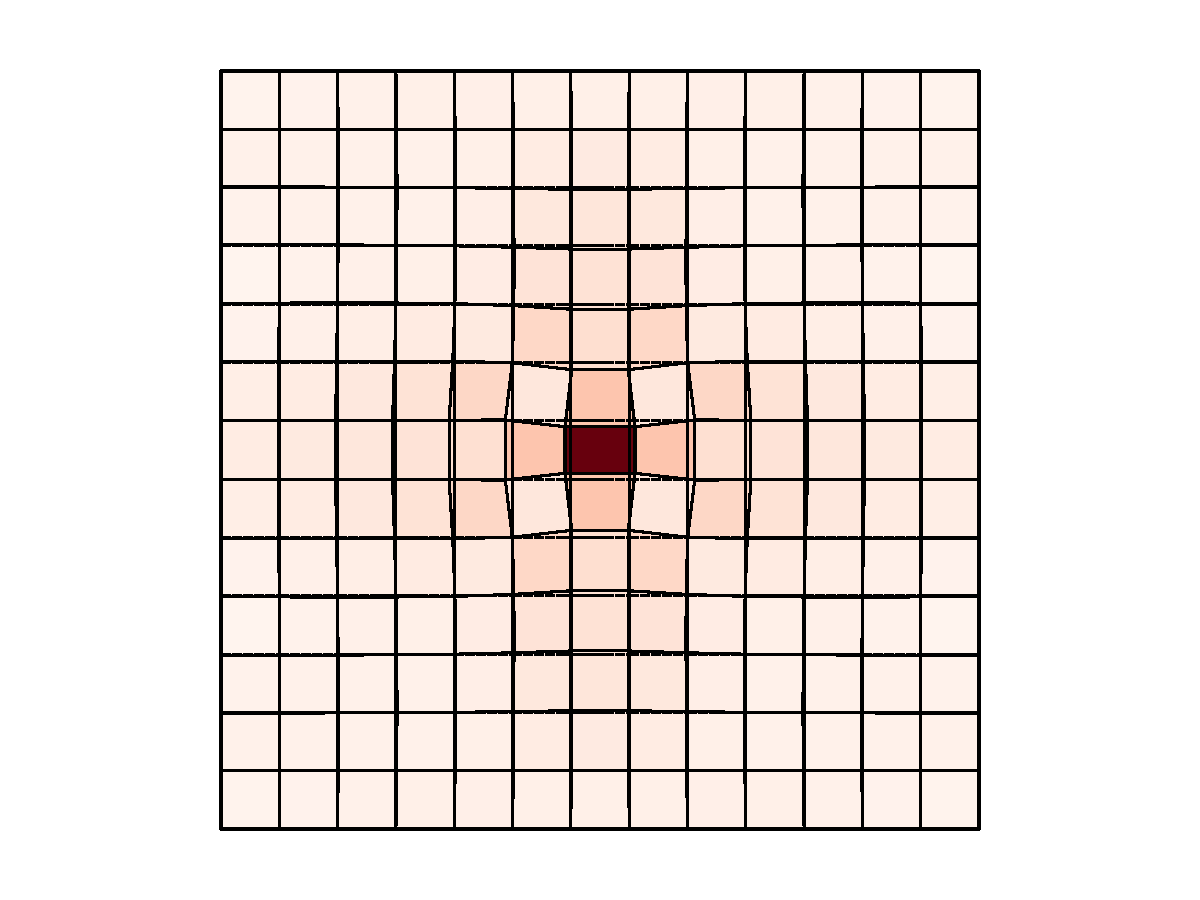
\includegraphics[width=\textwidth]{perturbation_pure-shear.pdf}
        \subcaption{Pure shear}
        \label{fig:perturbation:pure-shear}
    \end{minipage}
    \caption{
        Perturbation modes.
        The shown colour is the equivalent deviatoric stress resulting from the perturbation.
    }
    \label{fig:perturbation}
\end{figure}

\begin{figure}[htp]
    \centering
    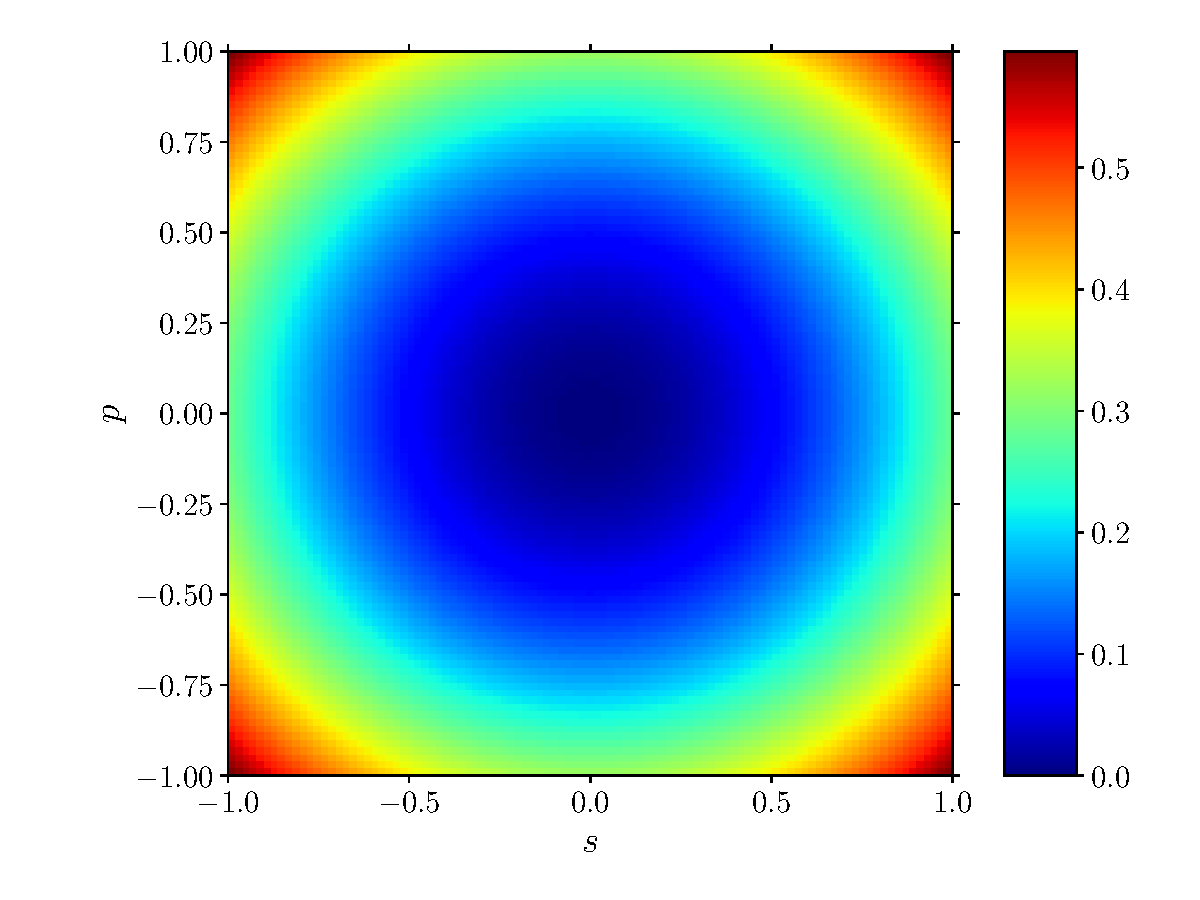
\includegraphics[width=.5\textwidth]{phase-diagram_energy.pdf}
    \caption{
        Energetic cost of a perturbation:
        $\delta \vec{u}(\vec{r}) = s \vec{u}_s (\vec{r}) + p \vec{u}_p (\vec{r})$.
    }
    \label{fig:energy}
\end{figure}

\begin{figure}[htp]
    \centering
    \captionsetup[subfigure]{justification=centering}
    \begin{minipage}[t]{.49\textwidth}
        \centering
        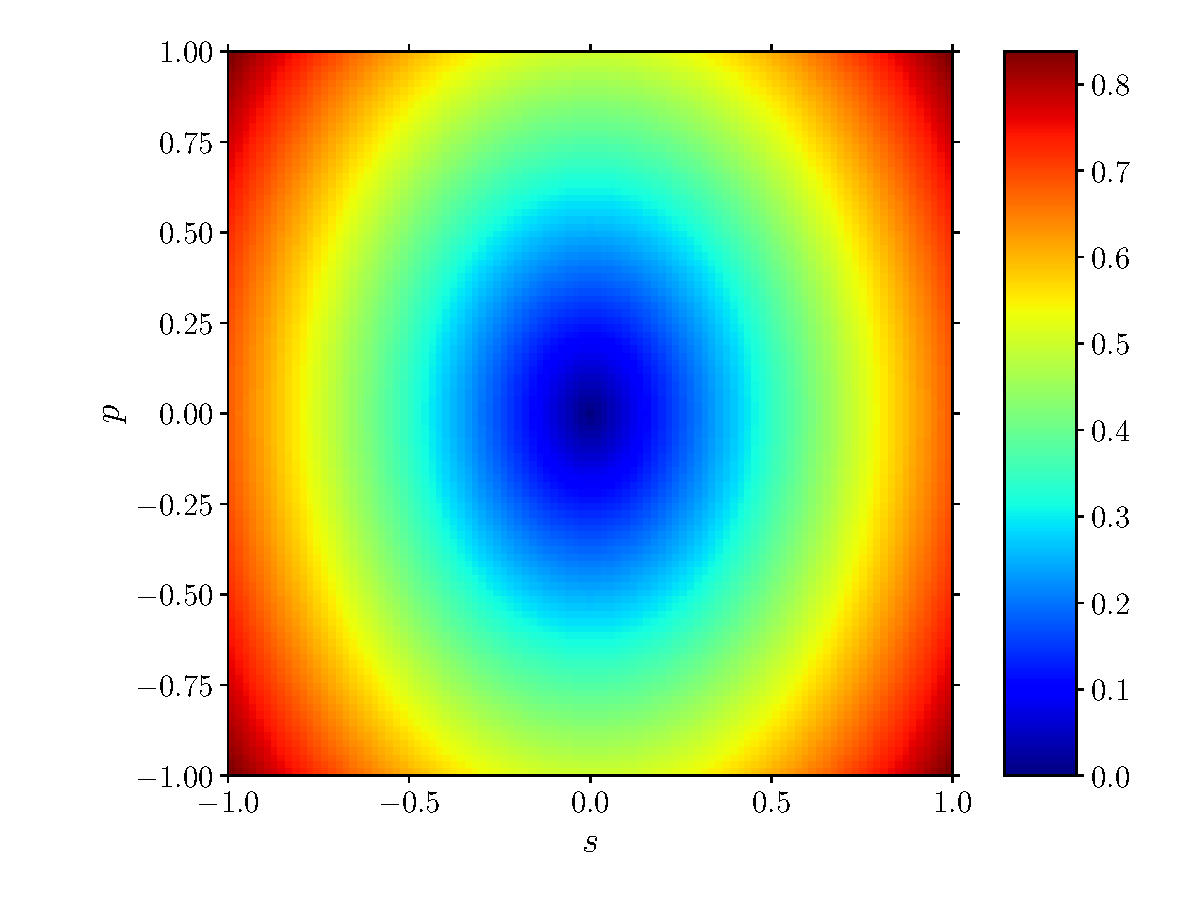
\includegraphics[width=\textwidth]{phase-diagram_sig.pdf}
        \subcaption{
            Equivalent stress.
        }
        \label{fig:phase-diagram:sig}
    \end{minipage}
    \hfill
    \begin{minipage}[t]{.49\textwidth}
        \centering
        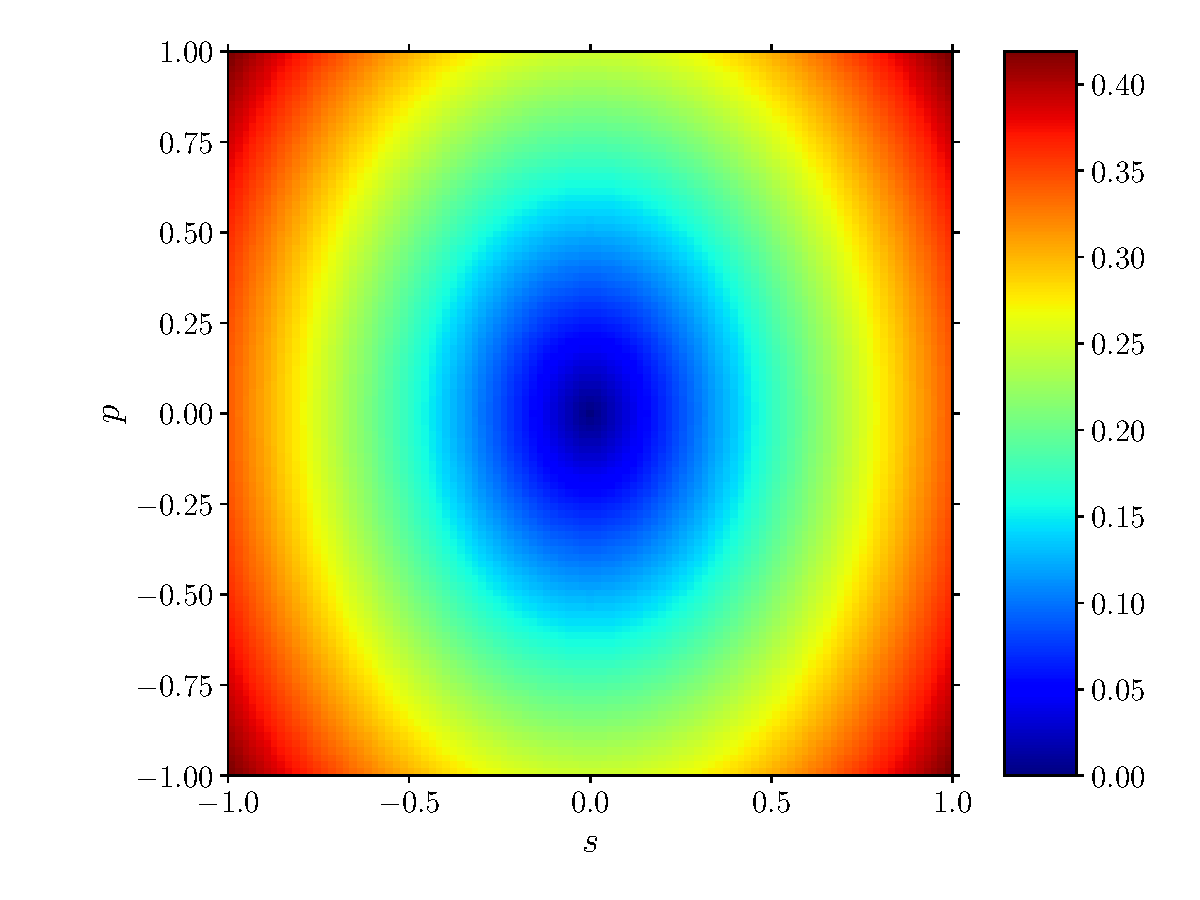
\includegraphics[width=\textwidth]{phase-diagram_eps.pdf}
        \subcaption{
            Equivalent strain.
        }
        \label{fig:phase-diagram:eps}
    \end{minipage}
    \caption{
        Resulting
        \subref{fig:phase-diagram:sig} equivalent stress and
        \subref{fig:phase-diagram:eps} equivalent strain
        for a perturbation:
        $\delta \vec{u}(\vec{r}) = s \vec{u}_s (\vec{r}) + p \vec{u}_p (\vec{r})$.
    }
    \label{fig:phase-diagram}
\end{figure}

\clearpage

\section*{Example}

As an example a configuration is considered in which an elastic medium is subjected
to a shear deformation of the top boundary and a random prestress along the middle layer.
The resulting equilibrium configuration is shown in \cref{fig:example:start}.

An element is then selected for triggering such that the equivalent strain in the element
increases to some value $\varepsilon_y$.
For the described protocol the perturbation of minimal energy, results in the following
strain tensor in the triggered element
\begin{equation}
    \bm{\varepsilon} =
    \begin{bmatrix}
        E_0 & \gamma_0 \\
        \gamma_0 & - E_0
    \end{bmatrix}
    + \eta
    \begin{bmatrix}
        \delta E & \delta \gamma \\
        \delta \gamma & - \delta E
    \end{bmatrix}
\end{equation}
where $\eta = s = p$ thus follows as the solution of
\begin{equation}
    \varepsilon_y^2 = (E_0 + \eta \delta E)^2 + (\gamma_0 + \eta \delta \gamma)^2
\end{equation}
The perturbation is shown in \cref{fig:example:perturbation} and the perturbed configuration
where the equivalent strain in the triggered element is equal to $\varepsilon_y$ is shown
in \cref{fig:example:end}.

\begin{figure}[htp]
    \centering
    \captionsetup[subfigure]{justification=centering}
    \begin{minipage}[t]{.3\textwidth}
        \centering
        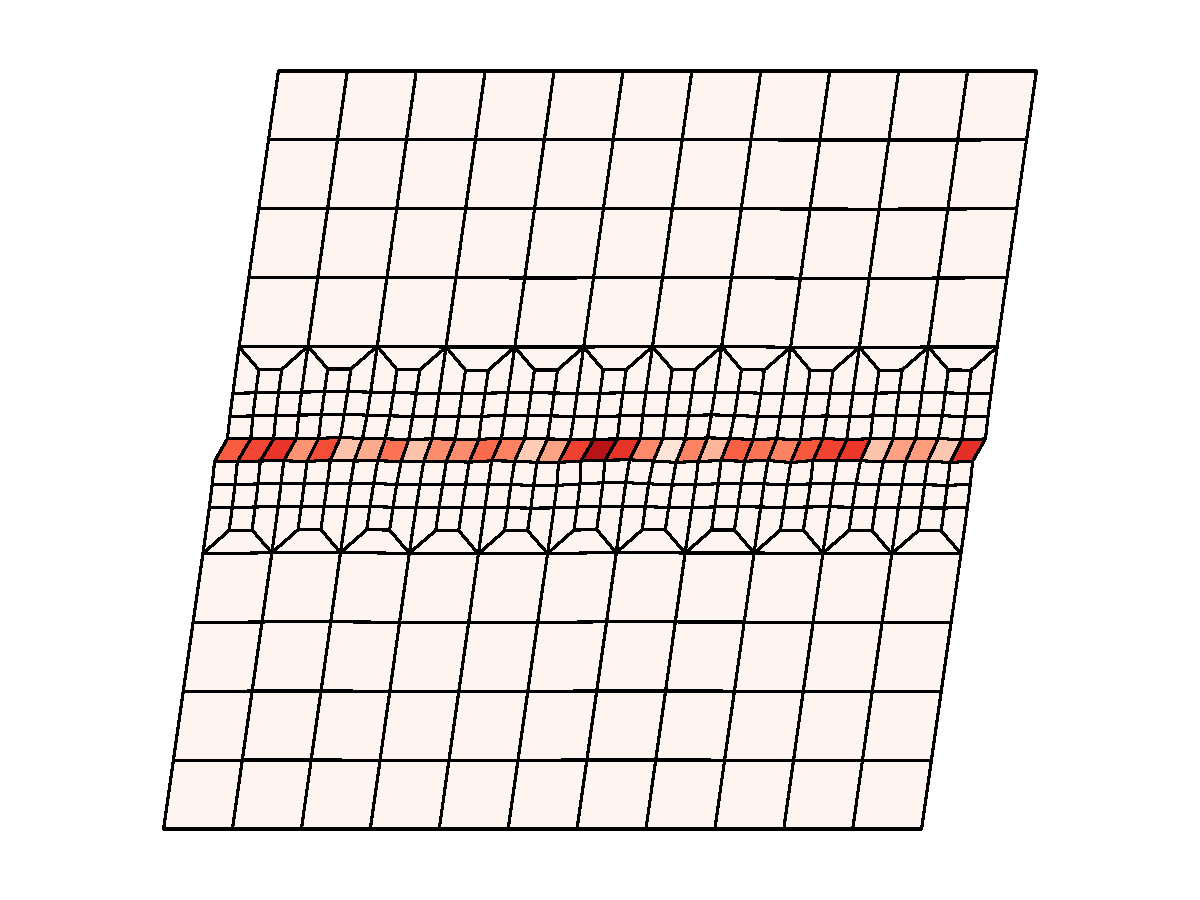
\includegraphics[width=\textwidth]{example_start.pdf}
        \subcaption{Starting configuration.}
        \label{fig:example:start}
    \end{minipage}
    \hfill
    \begin{minipage}[t]{.3\textwidth}
        \centering
        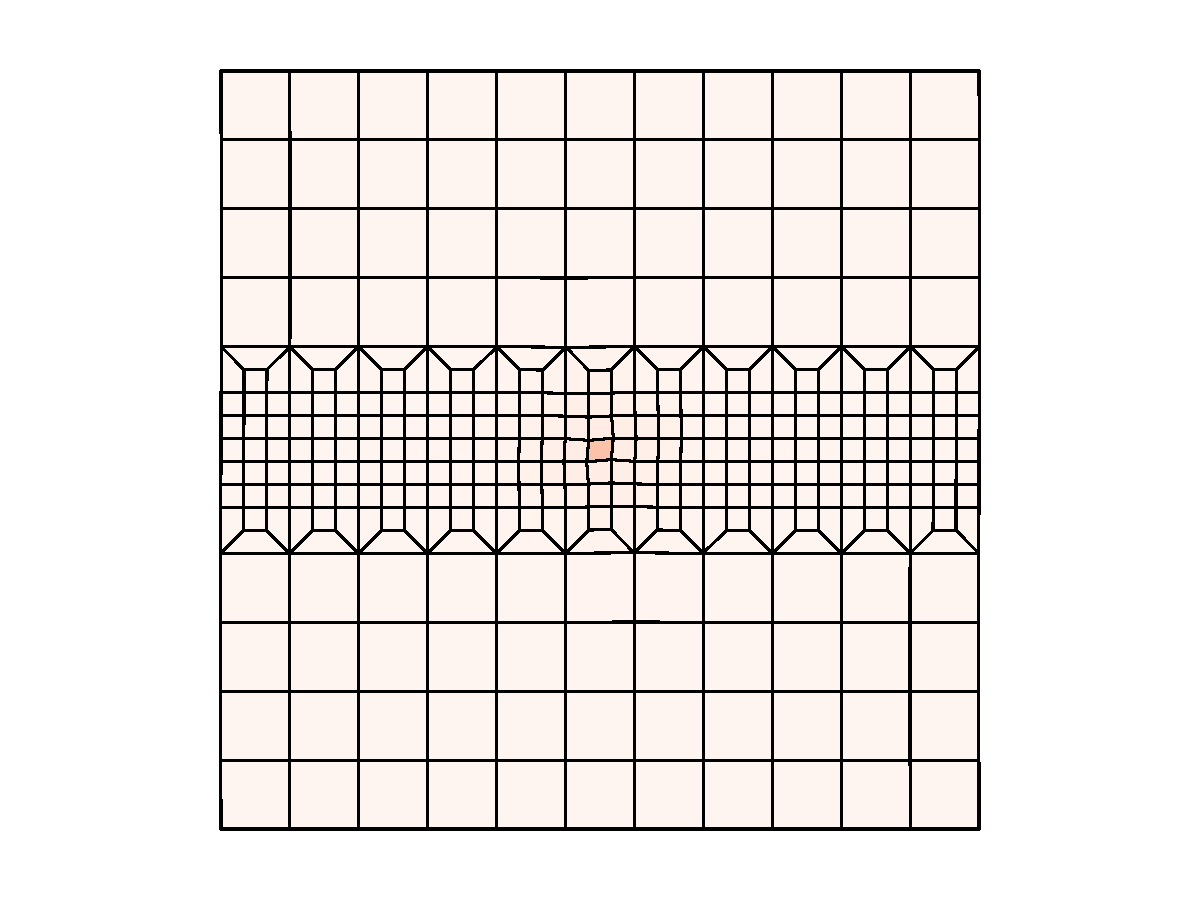
\includegraphics[width=\textwidth]{example_perturbation.pdf}
        \subcaption{Applied perturbation.}
        \label{fig:example:perturbation}
    \end{minipage}
    \hfill
    \begin{minipage}[t]{.3\textwidth}
        \centering
        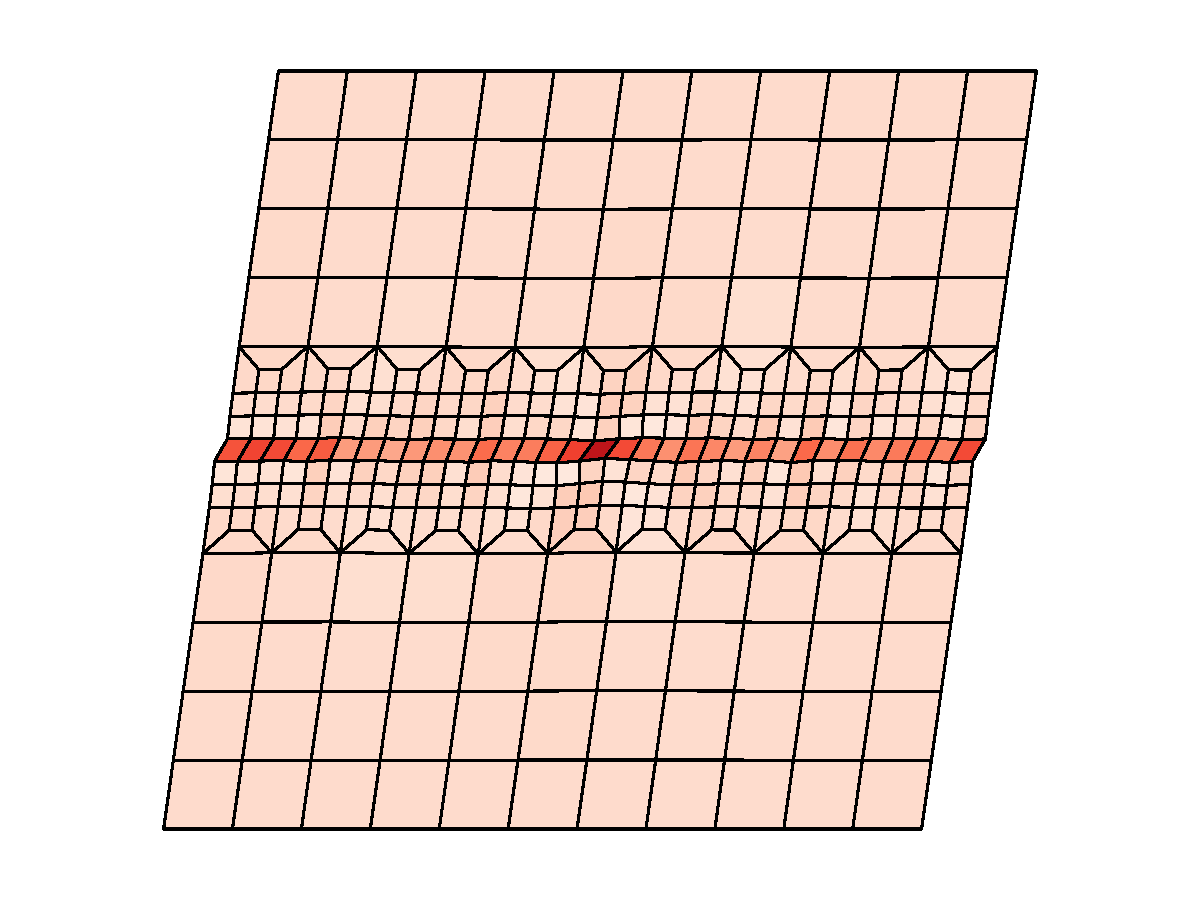
\includegraphics[width=\textwidth]{example_end.pdf}
        \subcaption{Perturbed starting configuration.}
        \label{fig:example:end}
    \end{minipage}
    \hfill
    \caption{Friction-like example.}
    \label{fig:}
\end{figure}
{}


\end{document}
